\documentclass[a4paper,10.0pt,twoside]{npr}

\usepackage{multicol,graphicx,lastpage,footmisc,fancyhdr,paralist,
tabularx,array,booktabs,caption,multirow,upgreek,mathrsfs,gensymb,color}
\usepackage[fancyhdr,space,fntef,fontset=ubuntu]{ctex}
\usepackage{amssymb,bm,mathrsfs,bbm,amscd}
\usepackage{flushend,cuted}
\usepackage{refcount}
\usepackage{savesym}
\usepackage{textcomp}
\usepackage[tbtags]{amsmath}  %
\savesymbol{iint}
\usepackage{amstext} %数学宏包文本命令
\usepackage{balance} %版心底部对齐

\flushbottom      %版心底部对齐
\setcounter{section}{0}
\begin{document}
%\begin{CJK*}{GBK}{\song}{\wuhao}{\rm}

%___________________________________________________________________________________
\def\rd{{\rm d}}

\newcommand{\RM}{\ensuremath{\mathrm}}   %正体 既可用于文本模式也可用于数学模式
\newcommand{\dif}{\mathrm{d}}  %直立体d
\newcommand{\me}{\mathrm{e}}  %直立体e
\newcommand{\mi}{\mathrm{i}}  %直立体i
\newcommand{\mj}{\mathrm{j}}  %直立体j
\newcommand{\afrac}[2]{\dfrac{\,#1\,}{\,#2\,}}  %略长分数线
\newcommand{\nn}{\nonumber}  %公式无编号
\newcommand{\nt}{\noindent}
\newcommand{\OO}{~\text{。}}
\newcommand{\PP}{~\text{,}}
\newcommand{\OP}{~\text{;}}
\newcommand{\LT}{\left}
\newcommand{\RT}{\right}

%___________________________________________________________________________________

\balance
\fancypagestyle{myfoot}
{%
\fancyhf{}
\fancyhead[c]{\wuhao\song 高~等~核~物~理~实~验}
\renewcommand{\headrule}{\vskip 2pt
\hrule height0.4pt width\headwidth \vskip1pt
\hrule height0.4pt width\headwidth \vskip-1.8pt}
}%
\thispagestyle{myfoot}

%%%%%%%%%%%%%%%%%%%%%%%%%%%%%%%%%%%%%%%%%%%%%%%%%%%%%
%    奇偶页眉
%%%%%%%%%%%%%%%%%%%%%%%%%%%%%%%%%%%%%%%%%%%%%%%%%%%%%
\pagestyle{fancy}
\fancyhead{}
\fancyhead[ce]{\xiaowu\song \hspace{0.5em}高~等~核~物~理~实~验}
%\fancyhead[ro,le]{\xiaowuhao \hspace{0.5em}\textbf{\textperiodcentered}\;\thepage\;\textbf{\textperiodcentered}\hspace{0.5em}}
%\fancyhead[ce]{\xiaowu\song 粒~子~物~理~与~原~子~核~物~理~专~题~实~验}
%\fancyhead[re]{\xiaowu\song \hspace{0.5em}第\;31\;卷\hspace{0.5em}}
\fancyfoot[ce,co]{}
\renewcommand{\headrule}{\vskip 2pt
\hrule height0.4pt width\headwidth}


\setcounter{page}{001}%
\fancyhead[co]{\xiaowuhao\song  乔颢:用$^1$H($^{19}$F,$^{16}$O$^*$)$\alpha$反应分析氢分布}    %奇页页眉
\begin{center}
\title{%
\xiaoerhao \bf  %章标题为两行时改为 \exiaoer
用$^1$H($^{19}$F,$^{16}$O$^*$)$\alpha$反应分析氢分布\\[-5mm]}
\maketitle
\large \fs
乔颢$^{^1}$\\[2mm]

\xiaowu \song
1. 北京大学物理学院,海淀区 北京 100871;\\[4mm]

 
\footnotetext[0]{{\bf 作者简介:}~~\begin{minipage}[t][4.2mm]{149mm}\song
乔颢,E-mail: i@catofes.com
\end{minipage} }
%\footnotetext[0]{{\bf 通信作者:}\song ~~E-mail: xxx@xxx.xxx }%通信作者为第一作者时不要此项

\end{center}
%%%%6.正文
\vspace{5mm}
%%%%6.正文
\setcounter{section}{0}
\begin{multicols}{2}
%----------------
%____________________________________________________________________________
%%%%以上请不要改动%%%%%%%%%%%%%%%%%%%%%%%%%%%%%%%%%%%%%%%%%%%%
\section{原理}
\vspace*{-1mm}
\song\wuhao
1、共振核反应选择\\
本实验采用$^1$H($^{19}$F,$^{16}$O$^*$)$\alpha$共振核反应来测量氢在样品中的分布。
\begin{center}
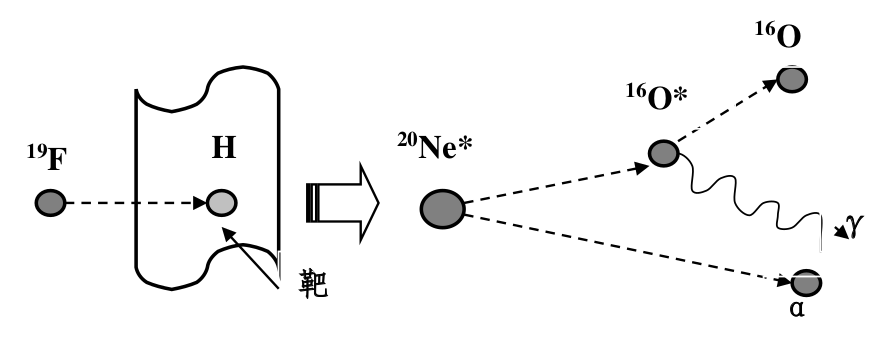
\includegraphics[width=0.4\textwidth]{1.png}
\\
\xiaowu\song 图~1\begin{minipage}[t]{75mm} \quad $^1$H($^{19}$F,$^{16}$O$^*$)$\alpha$共振核反应\\[-1mm]\wuhao
\end{minipage}
\end{center}
入射粒子$^{19}$F轰击靶核,生成处于激发态的$^{20}$Ne$^*$核,它退激后发射$\alpha$粒子和处于激发态的$^{16}$O$^*$核,$^{16}$O$^*$核退激后回到基态同时发射$\gamma$光子。该共振态的末态有$\alpha$和$\gamma$粒子。测量必须在真空下进行。我们只需测量$^{16}$O$^*$核退激发射的$\gamma$光子产额,以确定样品中氢的含量。\\
反应截面随入射粒子能量变化的曲线称为核反应的激发曲线。$^1$H($^{19}$F,$^{16}$O$^*$)$\alpha$的激发曲线如图所示。
\begin{center}
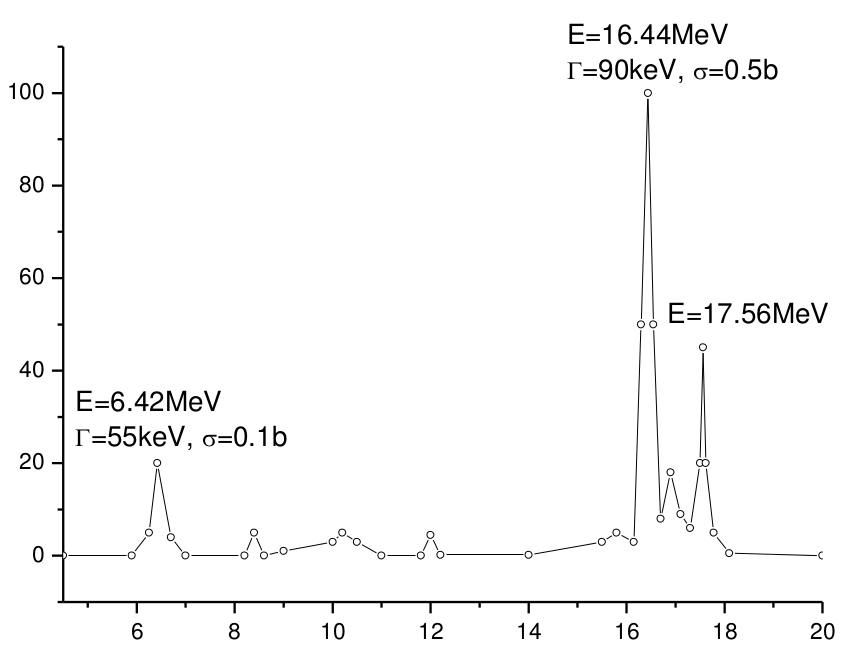
\includegraphics[width=0.4\textwidth]{2.png}
\\
\xiaowu\song 图~2\begin{minipage}[t]{75mm} \quad $^1$H($^{19}$F,$^{16}$O$^*$)$\alpha$共振核反应激发曲线\\[-1mm]\wuhao
\end{minipage}
\end{center}
对不同的入射离子能量,该核反应主要有两个主要的共振峰,分别在6.42MeV和16.44MeV。共振峰的形状用Breit-Wigner公式描述:
\begin{equation}
\sigma (E)=\frac{\sigma _R}{1+(\frac{E-E_R}{\Gamma /2})^2}
\end{equation}
其中$\Gamma$为共振峰宽度,E$_R$为共振能量,$\sigma$$_R$为共振截面。实验采用6.42MeV的共振($\Gamma$=55keV,$\sigma$=0.1b)测量氢分布。\\
6.42MeV的共振核反应产生的$^{16}$O处于激发态,退激时发出能量分别为6.13,6.92,7.12MeV的$\gamma$光子其中6.13MeV的光子的分支比为97\%,因此测量时不考虑其他两种光子。\\
2、氢分布分析原理\\
入射能量为E$_0$(高于共振能量)的F离子打到样品上,进入样品后逐渐损失能量。设在深度x处,F离子的能量损失了$\Delta$E后变为E。
\begin{center}
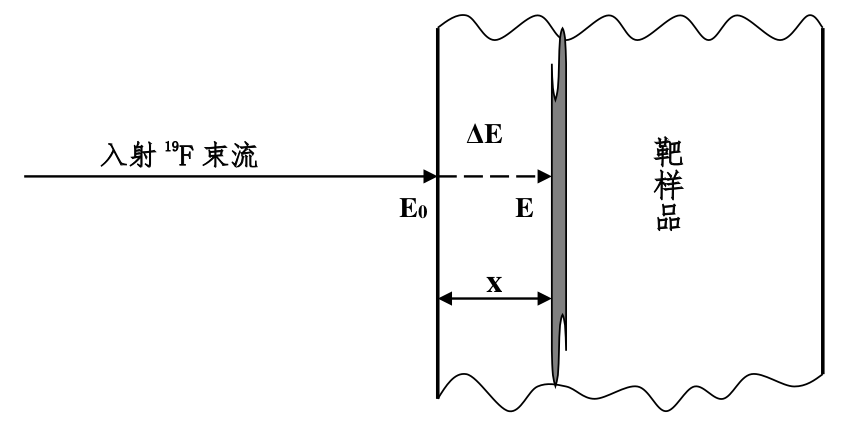
\includegraphics[width=0.4\textwidth]{3.png}
\\
\xiaowu\song 图~3\begin{minipage}[t]{75mm} \quad 氢分布分析示意图\\[-1mm]\wuhao
\end{minipage}
\end{center}
a、深度分析\\
F离子只有其能量为E$_R$时才和样品中的氢发生反应,
\begin{equation}
E=E_0-\Delta E \approx E_0-\left| \frac{dE}{dx} \right| \times x=E_R
\end{equation}
因此发生核反应的深度x为:
\begin{equation}
x=\frac{E_0-E_R}{\left| \frac{dE}{dx} \right| }
\end{equation}
F离子束流能量E$_0$和加速器高压的关系为E$_0$=HV$\times$(4+1)MeV,则
\begin{equation}
x(A)=\frac{[HV\times (4+1)-6.42]\times 10^6 (eV)}{\left| dE/dx \right| (eV/A)}
\end{equation}
改变加速器能量HV,不同入射能量的F离子就会和不同深度的氢发生核反应,记录反应后产生的光子产额,就可以得到样品中的氢分布。\\
b、含量分析\\
假设标准样品中,氢沿深度均匀分布,且氢含量C$_{st}$已知,测得$\gamma$光子计数为N$_{st}$,测得未知样品中的$\gamma$光子数为N;则待测样品的氢含量为
\begin{equation}
C=C_{st}\times \frac{\left| \frac{dE}{dx} \right|_{E=E_R} \times N}{\left| \frac{dE}{dx} \right|_{st(E=E_R)} \times N_{st}}\times \frac{\rho _{st}}{A_{st}}\times \frac{A}{\rho}
\end{equation}
对公式5的理解:\\
探测到的$\gamma$光子的数量N可以写为
\begin{equation}
N=\frac{\phi _F S\sigma C\rho}{A}\times dx
\end{equation}
其中$\phi$$_F$为入射F离子数量,$\sigma$为反应截面,S为束流面积,dx为在材料中能发生反应的厚度。设在共振能量$\Delta$E$_R$的范围内能发生反应,则dx=$\frac{\Delta E_R}{\left| dE/dx \right|_{E=E_r}}$。因此可以得到式5。

\section{实验步骤}
1、测量标准样品\\
标准样品所含的氢均匀分布在2$\mu$m的非晶硅层,含氢原子比为13.9\%。标准样品的测量数据如下:
\begin{center}
\bgliu
{\bf 表~1\quad
标准样品测量数据}\\[0.5mm]
\renewcommand{\arraystretch}{1.4}
\liuhao\song\rm
\newcolumntype{M}{>{\centering\arraybackslash}m{12mm} >{\centering\arraybackslash}m{12mm}>{\centering\arraybackslash}m{12mm}>{\centering\arraybackslash}m{12mm}}
\begin{tabular}{M}
\specialrule{0.1em}{0.1pt}{0.1pt}

电压/MV   &  电流/nA &  时间/s  &  计数 \\
\midrule
1.30  &  260   &  77 &  2294  \\
1.35  &  260   &  75 &  2310  \\
1.40  &  260   &  80 &  2415  \\
1.45  &  260   &  76 &  2336  \\
1.50  &  260   &  78 &  2545  \\
\specialrule{0.1em}{0.1pt}{0.1pt}
\end{tabular}\\
\renewcommand{\arraystretch}{1.0}
\end{center}

2、测量待测样品(样品10)

10号待测样品是不锈钢,具体的测量数据如下表所示:

\begin{center}
\bgliu
{\bf 表~2\quad
10号待测样品测量数据}\\[0.5mm]
\renewcommand{\arraystretch}{1.4}
\liuhao\song\rm
\newcolumntype{M}{>{\centering\arraybackslash}m{12mm} >{\centering\arraybackslash}m{12mm}>{\centering\arraybackslash}m{12mm}>{\centering\arraybackslash}m{12mm}}
\begin{tabular}{M}
\specialrule{0.1em}{0.1pt}{0.1pt}

电压/MV   &  电流/nA &  时间/s  &  计数 \\
\midrule
1.26  &  260   &  78 &  176   \\
1.29  &  225   &  89 &  1467  \\
1.32  &  270   &  78 &  1199  \\
1.35  &  270   &  77 &  1102  \\
1.38  &  280   &  72 &  835   \\
1.41  &  300   &  68 &  288   \\
1.44  &  310   &  66 &  99 \\
\specialrule{0.1em}{0.1pt}{0.1pt}
\end{tabular}\\
\renewcommand{\arraystretch}{1.0}
\end{center}

\section{数据分析}

首先是对标准样品的分析。标准样品的含H量为13.9\%,利用SRIM程序可以得到能损本领和能量之间的关系。cubic插值之后可以得到在我们感兴趣的6.42MeV能量处的能损。能损为173.28eV/A。

标准样品的H分布是均匀的,所以可以得到其平均计数为2380。因此可以得到公式5中的各个参数。有
$$C_{st}=0.139$$
$$N_{st}=2380$$
$$|\frac{dE}{dx}|_{st(E=E_R)} = 173.28eV/A$$
$$\rho_{st}=2.0085$$
$$A_{st}=24.147$$

因此可以根据公式5来计算待测样品的具体结果。当电压为1.26MV时加速器得到的能量小于共振能量,因而不会发生共振,所以不与考虑,其他电压情况下可以根据迭代法得到氢含量和电压的关系,数据表如下所示:

\begin{center}
\bgliu
{\bf 表~3\quad
10号待测样品氢含量信息}\\[0.5mm]
\renewcommand{\arraystretch}{1.4}
\liuhao\song\rm
\newcolumntype{M}{>{\centering\arraybackslash}m{12mm} >{\centering\arraybackslash}m{12mm}>{\centering\arraybackslash}m{12mm}>{\centering\arraybackslash}m{12mm}}
\begin{tabular}{M}
\specialrule{0.1em}{0.1pt}{0.1pt}

电压/MeV   &  氢含量/\%   &  能损本领/$eV\cdot A^{-1}$  & 对应深度/A   \\
1.26  &  -  &  -    & -  \\
1.29  &  12.26 &  426.6900  &  70.31 \\
1.32  &  10.25 &  434.9050  &  413.88   \\
1.35  &  9.49  &  438.0130  &  753.40   \\
1.38  &  7.33  &  446.8270  &  1074.24  \\
1.41  &  2.64  &  466.1560  &  1351.48  \\
1.44  &  0.92  &  473.2780  &  1648.08  \\
\specialrule{0.1em}{0.1pt}{0.1pt}
\end{tabular}\\
\renewcommand{\arraystretch}{1.0}
\end{center}

由此可以得到样品的氢含量,可以看到随着深度逐渐的加深,氢含量急剧的减少。这样符合待测样品(不锈钢)的特性。

\section{参考文献}

\noindent
[1] Peking Unviersity, Fudan University \ Nuclear Experment
\ Nuclear Publishing House, 1989 (in Chinese)

\noindent
 (北京大学,复旦大学.\ 原子核实验\ 原子能出版社,\ 1989)

\end{multicols}

\newpage

\clearpage
%\end{CJK*}
\end{document}

